% Import Packages
\documentclass[12pt]{article}
\usepackage[utf8]{inputenc}
\usepackage[table]{xcolor}
\usepackage{listings}
\usepackage[letterpaper, margin=1in]{geometry}
\usepackage{graphicx}
\usepackage{verbatim}
\usepackage{underscore}
\usepackage{fancyhdr}
\usepackage{hyperref}
\usepackage{enumitem}
\usepackage{hanging}
\usepackage{seqsplit}
\usepackage{multirow}
\usepackage{multicol}
\usepackage{array}
\usepackage{longtable}
\usepackage{xurl}

% Command for quick and easy bibliography
\newcommand\hangingindent[1]{\begin{hangparas}{0.5in}{1} #1 \end{hangparas}\vspace{0.5cm}}

% Command for coloring a table cell light gray and emboldening the text
\newcommand\cellhead[1]{\cellcolor{lightgray}\textbf{ #1 }}

% Change the color of hyperlinks to blue
\renewcommand\UrlFont{\color{blue}}

\pagestyle{fancy}
\fancyhf{}
\fancyhead[R]{Wall Guys: Assignment 5}
\fancyhead[L]{}
\fancyfoot[C]{\thepage}

\begin{document}

    \begin{titlepage}
        \begin{center}
            \vspace*{1cm}
            \Huge\textbf{ECE 396: Assignment 5}

                \vspace{0.5cm}
                \LARGE Wallcopter Project
    
            \vspace{1.5cm}
            \textbf{Team 13: Wall Guys}

                \vspace{0.5cm}
                Tien Dao, Hardik Goel, Jaden Mossman, and Anand Pudi

                \Large
                Sponsor: Dr Ahmet Enis Cetin

                Instructor: Dr Matthew Alonso

                \LARGE

            \vfill             
            \includegraphics[width=0.4\textwidth]{resources/uic_logo.png}

            % ASSIGNMENT DESCRIPTION
            \vspace{0.8cm}
            University of Illinois Chicago\\
            Fall 2022
                
        \end{center}
    \end{titlepage}

    \tableofcontents

    \newpage
    \section{Abstract}
        High rise buildings and the undersides of bridges are important structures that need to be examined for safety purposes, but this is often a difficult task as they are hard to reach places and typically experience high wind.
        Even when reached, the unstable environment often causes the resulting images used for inspections to be blurry and difficult to analyze.
        The aim of the project was to identify an accessible drone platform, modify it for inspections, and maintain control to collect data with the drone at typical heights and environmental conditions.
        The drone has an additional attachment that includes a camera and sensors that will assist the drone in taking pictures.
        Additionally, there are slide attachments atop the drone, which allow it to make contact with the upper surface and remain stable.
        All of these factors together allow us to obtain a stable image used for inspections.
        The captured images will be sent to a receiving computer, where an image-detecting algorithm will detect any cracks or damages.
        We have used the DJI Tello and ESP 32 microcontroller for the project and have included additional prop guards to allow the drone to ceilings periodically.
        Our accomplishments include successfully designing and building the drone prototype, incorporating the necessary components, and testing its functionality in stable flight.
        After inspecting some nearby structures we were able to test the range and image quality of the pictures providing a cost-effective solution to structural engineers and those responsible for ensuring the safety of these structures.
        This inspection run can be found with the videos that we recorded.
    
    \newpage
    \section{Overview}

        \subsection{Project Goals}
            The aim of this project is to develop an attachment onto a drone to allow additional features for inspection purposes.
            These inspections will be done in hard to reach places like under bridges or high rise buildings.
            We are looking to make at least a prototype that can go up to the ceilings of most areas and can navigate via a wireless control system.
            Our priority is as follows: main focus on functionality, producing a minimum working prototype, and then try to reduce the cost of the drone itself if possible.

        \subsection{Needs Statement}
            High rise buildings and the undersides of bridges are important structures that need to be examined for safety purposes, but this is often a difficult task as they are hard to reach places and typically windy and tough environments.
            Drones are often deployed to conduct these examinations, but there are limitations to their performance when coming into close contact with those surfaces.
            Another limitation is the lack of stable connection when the drone is a certain distance away from the user.
            These limitations, among others, provide a challenge to the autonomous examination of bridges and buildings.

        \subsection{Objective Statement}
            The objective of this project is the design of a drone that is able to navigate in a stable manner while remaining its set distance to the ceiling or object it is touching.
            The drone will have a camera installed that can capture images or give live feed for inspection purposes.
            Sensors will be used in order to calculate and articulate the distance between the drone and the ceiling.
            Standard wireless communication will be through the microcontroller that allows the user to control the device from a distance.

        \newpage
        \subsection{Background}
            \begin{enumerate}[label=\Alph*.]
                \item The basic concept that lays behind this wall-copter relies on the control system that keeps the copter stable to prevent collision or unintended side effect when approaching ceilings or walls.
                The current limitation lies on the unintended shifts of the blade speed when the copter gets too close to the wall's surface. 
                he other factor is the difficulty of control when the drone gets too close to such a surface.
                Surprisingly, there don't seem to be any current remedies that exist in the market right now, so we do not have a way to compare our project to it.
                Still, there are current market competitors who offer drones with strong frames that are used for inspections using LiDAR mapping technology.
                Those drones, whoever do not approach the ceilings or navigate close to the effect of rotors being sucked into a surface.
                They have to remain within a distance of 1.5 times the size of the rotor from the upper wall to remain safe and stable [1].
                There are other approaches to keeping the drone stable within these areas as there are studies focused on navigation via tilting the drone against the wall in order to ascend in a stable manner [2].
                This research focuses on scaling vertically using the Tilt Motor Mechanism that results in some successes in keeping the drone stabilized enough for certain tasks.
                An existing prototype exists for that research, but it does not seem like they have a focus on releasing that product into the market [2].
                One other alternative approach done by students from Shandong University of Science and Technology suggests creating a drone that would stick to walls/ceiling similar to geckos [4].
                This particular design focuses on solving the problem of inspection when natural disasters occur, which is only similar to our objective but the designs would be very beneficial to keep in mind.
                Once again, this is only a test product, not meant for release in the market and would not be our direct competitor.
                
                \indent Upon further background research, we found out that a license would be required in order to fly certain types of drone [5].
                Luckily, a license is not required for small indoor drones that are used for commercial purposes.
                So initial testing using indoor labs will not require such a license but will be different for outdoor tests.
                When looking into the drone market, typical drone prices vary quite a bit, from a very cheap price of \$30 that can go up to thousands [6].
                Usually the bigger the drone and more functionality it offers, the more expensive the product will be.
                So in order to remain competitive, our drone need to be within a reasonable range of around \$100-\$250, the amount that our budget would be allocated.
                
                \item Our background of this project is very clear from the beginning since it's a sponsored project, we still interviewed the professor to answer more questions we had.
                From this, we understand that the professor wants a product that currently does have strong competitors within the market space. 
                \begin{enumerate}[label=\roman*.]
                    \item Functionality: The goal is to make a drone which navigates in high places without the current problems (shaking, height limit close to ceiling, stability).
                    \item Appearance: It will look just like a common drone that currently exists in the market except with add-ons that would assist it with our goal.
                    \item Cost: The cost of the drone is preferred to be as low as possible since it is a commercial product.
                    For now our goal is just your standard drone cost that one can find for a reasonable price range of 40-100 dollars.
                    \item User Interface: Our user interface would be that of your standard drone control, but with potentially an extra set of control for the sets of wheels that will be at the top of the device.
                    \item Reliability: We want to obtain a product that will be consistent with every use.
                    This device should be very reliable since it builds upon the existing frame of a normal drone.
                    \item Power Requirements: The drone runs on a standard rechargeable battery which can also power our wheel system. Perhaps additional modification might be required if there is more power required to run the drone, but currently it would be safe to assume a standard drone battery would be able to run just fine also.
                    \item Expected Product Lifetime: As this kind of drone would be more difficult to navigate, we can assume it has a lower average product lifetime.
                    However, with proper use and care, it should still last only a little bit less if not the same amount of time as a standard drone.
                    \item Interfacing requirements with other systems.
                    \item User training needs: It is safe to assume that there will be a learning curve to the device in addition to learning how to navigate using the extra set of wheels on top.
                    Such a process can be learned just like a normal drone and should still be able to learn with some time and effort.
                    \item Government regulations and licensing: According to Part 107 of the FAA, any drone that weights over 250g needs to be registered even if it's only for commercial purposes.
                    This process shouldn't be too difficult and there isn't too much of a barrier to obtain one for use.
                    \item Industry standards: We follow the rules given to all drones.
                    Since our product is newer, we don't know what other standards might be applied to it.
                    So currently we'll be abiding by the current drone industry standards.
                    \item Safety issues: The drone has the issue of crashing into high terrains and falling onto passerby below.
                    There is also potential that objects that the wheels made contact with on the ceiling could potentially break and fall.
                    The device has the same safety problems as normal drones, only with additional unforeseen safety issues that come with driving it on the wall/ceiling.
                    \item Environmental Concerns: This device should be fairly safe environmentally to operate, with a low carbon footprint.
                    There are still concerns that when it crashes or is lost, if not recovered, it would be non-biodegradable as it is made out of plastics and other electronic components.
                    The battery that is used to operate the drone is also bad for the environment if not recycled correctly.
                \end{enumerate}
            \end{enumerate}
        \newpage

        \subsection{Marketing Requirements}
            For our marketing requirements, we focus on the standard requirements that most drones have.
            Additionally, we consider its cost-effectiveness along with the development cost of our design when making our requirements.
            We also include data from the interview that we had with our sponsor when making considerations of our marketing requirements.
            \begin{enumerate}[label=\arabic*.]
                \item The wall-copter must be able to climb on flat surfaces.
                \item The wall-copter should be stable.
                \item The wall-copter should be easy to use.
                \item The wall-copter should be cost-effective and easy to maintain.
                \item The wall-copter must be able to be controlled by a user from a distance.
                \item The wall-copter should be able to operate within a reasonable amount of time.
                \item The wall-copter should have minimal environmental impact.
                \item The wall-copter should follow proper regulations policies.
            \end{enumerate}
        
        \subsection{Objective Tree}
            There were many considerations when it came to our Objective Tree, we decided that there should be a split focus among maneuverability and stability, which both had high percentages.
            The ease of use would come as an extra priority in order to make it easier for our users to operate.
            The diagram below shows all the sub-focuses and their priority within each category.
            \centerline{\Large \underline{\textbf{Wall Copter}}}
            \begin{multicols}{3}
                \noindent\underline{Traversing Ceilings / Rough Surfaces 0.45}
                
                \noindent Walls 0.10
                
                \noindent Ceilings 0.70
                
                \noindent Underneath bridges 0.20

                \columnbreak

                \noindent\underline{Ease of Use 0.10}

                \noindent Limited controls 0.36

                \noindent Long operating time 0.64

                \columnbreak
                
                \noindent\underline{Be Stable 0.45}
                
                \noindent Sturdy structure 0.42
                
                \noindent Accurate motion sensors 0.35
                
                \noindent Long-lasting motors 0.23

            \end{multicols}
        
        \subsection{Additional Information}
            Upon further research, we found additional inspection drones that are available in the market [8].
            Those, however, are all very expensive as they are high-end drones that are usually manufactured for very specific tasks and are not flexible for its high price.
            On the high side of this, we have drones like the AscTec Falcon 8 that go up to \$48,000 in the market [9].
            Even on the low side, drones like the DJI Inspire 2 would still go up to \$3,299 [10].
            From this research, we also noted that there have yet to be any drones in the market with an elliptical ski design.
    
    \newpage
    \section{Engineering Requirements / Technical Specifications}
        \begin{longtable}{ | m{4.25cm} | m{5cm}| m{5.4cm} | }
            \hline
            Marketing Requirement & Engineering Requirement & Justification \\\hline
            1,2 &
            The wall-copter should be able to go to the heights of the ceiling, usually around at 20ft. &
            The product should adhere to the drone standard of being airworthiness (IEEE 1936.1-2021) \\\hline
            2 &
            The wall-copter should have standard drone speed of around 20 mph tops. &
            The device should be able to meet mechanical, and electrical requirements (IEEE 1937.1-2020) \\\hline
            4 &
            The device should be within a reasonable price range of around \$100-\$250. &
            Although there isn't a requirement for prices, the device should follow standards for estimating costs (IEEE 3001.4-2020)\\\hline
            6 &
            The wall-copter should be able to run for at least 10-15 minutes and is rechargeable. &
            The battery should follow IEEE guidelines for safety and usability (IEEE 1625-2008)\\\hline
            7 &
            The device should not emit any pollution and should not affect its surrounding environment too much. &
            The device should be following all the standards and remain environmentally sustainable (IEEE 1680.1) \\\hline
            3,5 &
            Users should be able to follow FAA regulations when operating the drone. &
            The user needs to be properly taught to operate the wall-copter in order to be safe for themselves and others (IEEE 1936.1-2021) \\\hline
            8 &
            The user needs to have the proper license needed in order to operate the device. &
            Qualification of operator is needed in order to use the product (IEEE 1936.1-2021) \\\hline
            4 &
            The drone blades and parts such as batteries and microcontroller/ sensors should be easily disconnected in order to clean/replace. &
            The device have to adhere to proper functionality for easy maintenance (IEEE 1937.1-2020) \\\hline
            4 &
            The wall-copter should be easy to make with additional modification to a standard drone production. &
            The product needs to be in line with manufacturing process control (IEEE 1625-2008) \\\hline
            1,2,3 &
            The wall-copter should be able to perform all tasks while maintaining a good lifespan of 150-800 flight hours. &
            The device should be very reliable in order for repeated use (IEEE 1680.1) \\\hline
            3,5 (including user interface) &
            The user should be able to operate the device after some basic training similar to how a normal drone should operate. &
            As the product require data to be collected for operations, it should also follow the drone data classification (IEEE 1936.1-2021) \\\hline
        \end{longtable}

        \subsection{Non-Applicable Parameters}
            Political: There isn't a current political aspect to our device as it is something that is used for inspection purposes.
            The only potential aspect would come from the privacy concerns that might come from the use of the drone for its unintended reason.
            That is something that every kind of drone would have by default.
            Since the locations our drone is made to inspect is hard reach in nature, we do not expect there to be any privacy issues.

            Social and Cultural: Our drone does not have any social and cultural features that would fit as an engineering requirement.
            Its uses are only intended for technical reasons and should not have any social related issues or any form of cultural influence.
    
    \newpage
    \section{Engineering Design Alternatives}
        \subsection{Design 1}
            This design includes an ultrasonic sensor in order to determine the distance between the drone and the ceiling/objects.
            We would have ball bearing wheels at the top in various selected locations.
            The drone would handle the movement both vertically and horizontally.
            In order to control the drone, we would be using a controller that communicates with the drone.
            The drone still would include a camera on top for image capturing.

            \vspace{0.5in}
            \centerline{\includegraphics{./resources/assignment3-Design1.schematic.drawio.pdf}}

            \vspace{0.5in}
            \begin{tabular}{|c|l|}
                \hline
                \multicolumn{2}{|c|}{\textbf{Design 1, Level 0}} \\\hline
                Module & Wall-Copter \\\hline
                \multirow{3}{3cm}{Inputs}
                    & - Power: Lithium Ion Battery\\
                    & - User Input by Controller \\
                    & - Sensor Data (Ultrasonic Sensor) \\
                    \hline
                \multirow{2}{3cm}{Outputs}
                    & - Drone Movement \\
                    & - Image Data Capturing \\
                    \hline
                \multirow{3}{3cm}{Functionality}
                    & - Precision flight control close to the roof through sensor data. \\
                    & - Movement along the roof with simple ball bearing wheels. \\
                    & - Capturing image for building inspections. \\
                    \hline
                
            \end{tabular}
            
        \newpage
        \subsection{Design 2}
            Using the idea of having two cameras (one on top, one built in) with an imaging system that would be used to determine the distance to the wall.
            Will use motorized wheels on top of the drone for horizontal navigation.
            
            \vspace{0.5in}
            \centerline{\includegraphics{./resources/assignment3-Design2.schematic.drawio.pdf}}

            \vspace{0.5in}
            \begin{tabular}{|c|l|}
                \hline
                \multicolumn{2}{|c|}{\textbf{Design 1, Level 0}} \\\hline
                Module & Wall-Copter \\\hline
                \multirow{3}{3cm}{Inputs}
                    & - Power: Lithium Ion Battery\\
                    & - User Input by Phone App \\
                    & - Imaging Data \\
                    \hline
                \multirow{3}{3cm}{Outputs}
                    & - Drone Movement \\
                    & - Wheel Movement \\
                    & - Image Data \& Video \\
                    \hline
                \multirow{4}{3cm}{Functionality}
                    & - Precision flight control close to the roof. \\
                    & - Capturing images and using them for computer vision flight control. \\
                    & - Live feedback of data through Wi-Fi. \\
                    & - Navigation on the roof through motorized wheels. \\
                    \hline
                
            \end{tabular}

        \newpage
        \subsection{Design 3}
            This design uses lasers placed in triangular configuration to triangulate the correct distance between the drone and the ceiling.
            It will also be using some kind of ski device to assist in movement at the ceiling or rough surfaces.
            The drone will also be controlled by a standard controller that comes with the product.

            \vspace{0.5in}
            \centerline{\includegraphics{./resources/assignment3-Design3.schematic.drawio.pdf}}

            \vspace{0.5in}
            \begin{tabular}{|c|l|}
                \hline
                \multicolumn{2}{|c|}{\textbf{Design 1, Level 0}} \\\hline
                Module & Wall-Copter \\\hline
                \multirow{3}{3cm}{Inputs}
                    & - Power: Lithium Ion Battery\\
                    & - User Input by Controller \\
                    & - Laser Sensors \\
                    \hline
                \multirow{2}{3cm}{Outputs}
                    & - Drone Movement \\
                    & - Image Data Capturing \\
                    \hline
                \multirow{3}{3cm}{Functionality}
                    & - Using sensor data for stabilized flight control close to the roof. \\
                    & - Capturing image for building inspections. \\
                    & - Using ski design to help device navigate at the top. \\
                    \hline
                
            \end{tabular}
            \newpage

        \subsection{Differences and Similarities Between Designs}
            Our three designs are very similar in principle as they all have the goal of detecting when the drone is close to the ceiling and giving feedback to the system.
            The designs were built upon this principle, keeping the drone from hitting the ceiling.
            They also have ways in which they navigate while touching the ceiling.
            They all share a control system in which we communicate to it through a controller, what we usually see in standard drones.
            Although these designs are similar, they are quite different as we try to create variations that can hopefully determine the best outcome.
            Their main differences are the sensors that go on them.
            Design 1 uses an ultrasonic sensor while Design 2 uses a camera with imaging processing and Design 3 uses lasers.
            Each of these variations have their own strengths and weaknesses that vary with costs.
            However, they all achieve the same goal of telling the drone if there's an object overtop of it (and how close) in order to avoid collision.
            Another difference is how the drone is going to navigate over the ceiling, with Design 1 using ball bearing wheels that would just serve as a way to move while Design 3 uses skis in order to slide while the drone itself performs the movement.
            In that case, movement will be handled by the drone itself, reducing the design complexity.
            Design 2 uses motorized wheels, which runs using its own motor, this will allow the drone to move without compromising its vertical movements.
            One last difference is how they are controlled, all would have the same communications via Wi-Fi with the main difference being that Design 1 and Design 3 using a standard drone controller, while Design 2 aims to use a phone app as its control.

    \newpage
    \section{Selection of Best Alternative Design}
        \subsection{Design Criteria}
            \begin{enumerate}
                \item \textbf{Development Cost}
                
                One of the main restrictions to a project, the amount of materials and the quality of the materials itself depend on this figure.
                We take our budget into consideration when comparing our development cost with other criteria.

                \item \textbf{The Group's Technical Knowledge about the Design Alternative}
                
                We are limited by what we and our advisor can cover with their expertise.
                The general goal is to keep it to something we can learn and realistically execute.
                Technical knowledge that is too complex to execute should be placed lower in priority.

                \item \textbf{Time Needed to Complete Design and Development}
                
                We should always keep our time limit in mind when it comes to making a design.
                Being mindful of our time limit is crucial for us to effectively achieve our goals.
                In this case, it is the end of the semester.

                \item \textbf{Suitability for Demo for 397}
                
                We should aim to get a prototype for our demonstration, so choose a design that is reasonable for making a prototype.
                Our prototype should be functional or at least most of it should be done for presentation within the expo.

                \item \textbf{Ease of Product Use}
                
                A product should always be easy to use or at least fairly achievable after minimal training in order to gain interests from the consumer.
                Keeping things in the lower side of the complexion will aid in usability and increase interest in the use of our product.
            \end{enumerate}
        
        \subsection{Final Decision Matrix}
            \noindent For additional tables, see Apppendix D.

            \begin{center}\begin{tabular}{|l|r|r|r|r|}
                \hline
                \cellhead{Criteria} & \cellhead{Avg Weight} & \cellhead{Design 1} & \cellhead{Design 2} & \cellhead{Design 3} \\\hline
                \cellhead{Dev Cost} & 0.189 & 4 & 2 & 3 \\\hline
                \cellhead{Knowledge}& 0.222 & 3 & 2 & 3 \\\hline
                \cellhead{Time Needed} & 0.258 & 4 & 2 & 3 \\\hline
                \cellhead{Demo} & 0.198 & 1 & 5 & 3 \\\hline
                \cellhead{Ease of Use} & 0.133 & 2 & 3 & 3 \\\hline
                & \cellhead{Score:} & 2.917 & 2.727 & 3 \\\hline
            \end{tabular}\end{center}
        
        \subsection{Final Decision}
            After collecting the data from each member, we obtained a personalized comparison of each of our criteria.
            These data were then analyzed to obtain the geometric mean and weights.
            We then compare these data in a pair-wise comparison table and get an average of our weights.
            This way, we know what the team thinks of each criteria overall, with Time Needed being the highest weight at 0.257 and knowledge coming second at 0.22.
            We then proceed with giving a score to all criteria based on the design as a group.
            Finally, we input the data into our Final Decision Matrix.
            To our expectation, design 3 has the highest score of 3 after all the calculations.
            What surprised us was how close design 2 is to winning, with the score being 2.92.
            It would also mean there are certain factors of design 2 that seem to work out within our criteria.
            After some analysis, we try to understand what is good and will be incorporating it into our design 3 for the best overall results.
            This design features lasers as our sensors and wheels overtop that seems to fit most of our preference, we will also be attempting to incorporate the demo capability of design 2 into it to improve our final design.

    \newpage

    \section{Preliminary Design}
        \subsection{Level 1 Schematic}
            \centerline{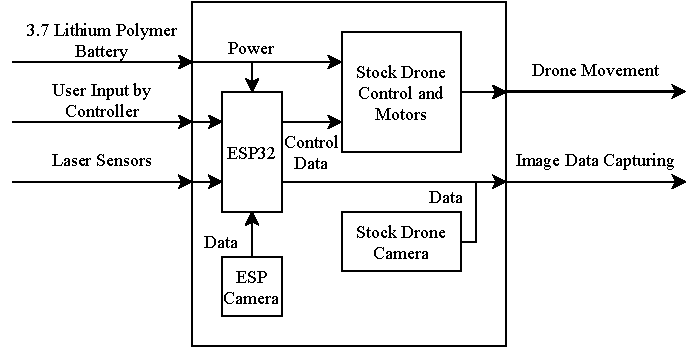
\includegraphics{./resources/level1.pdf}}
        \subsection{Circuit Diagram}
            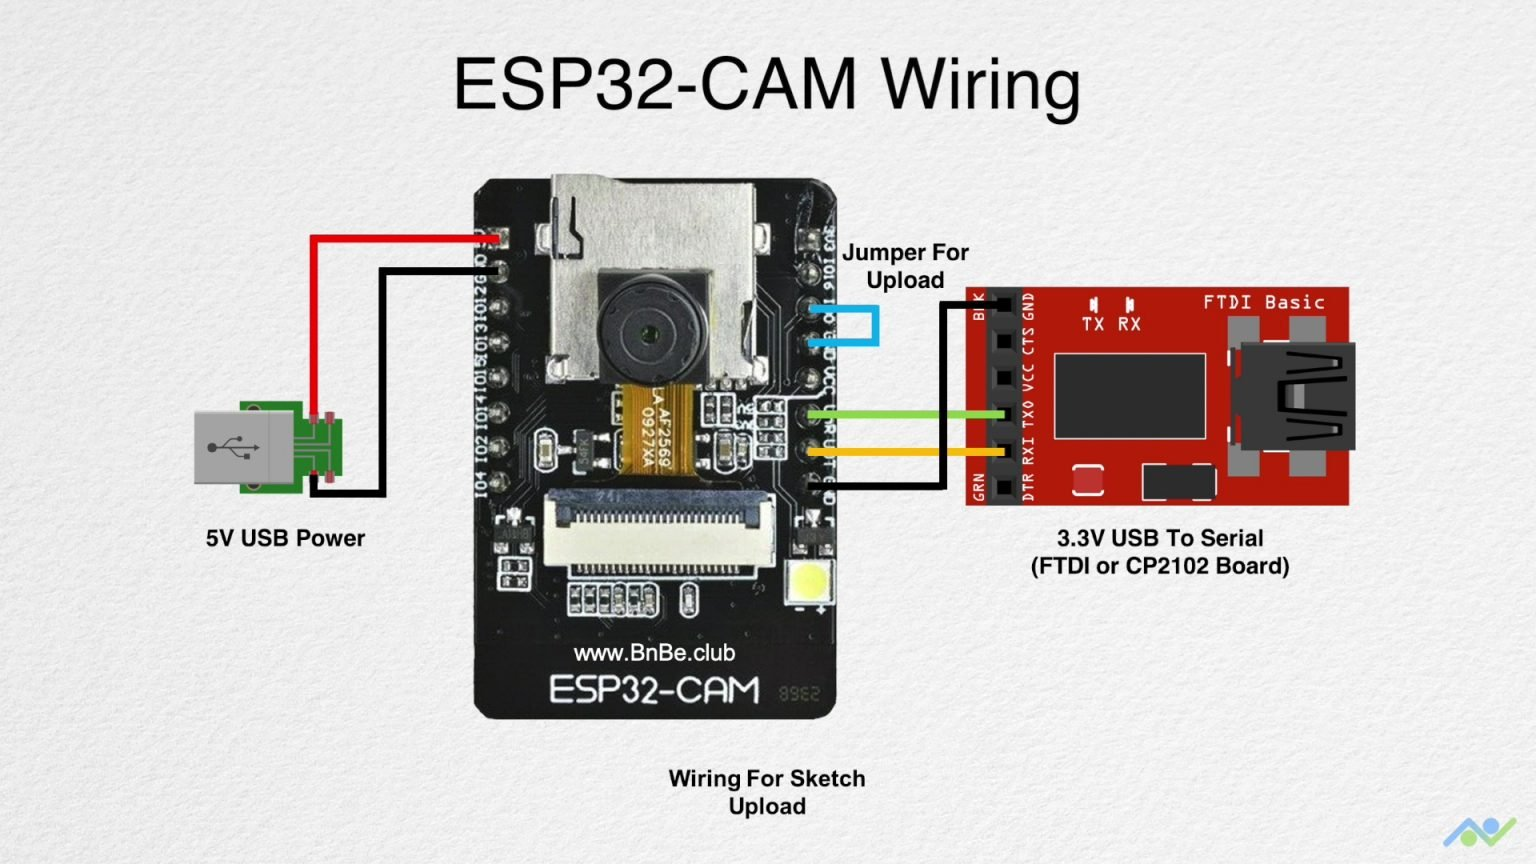
\includegraphics[width=0.4\textwidth]{resources/esp32cam_wiring.jpg}
        \subsection{Software Design}
    \newpage

    \section{Bibliography}
    \centerline{\large \underline{\textbf{Works Cited}}} \vspace{0.5cm}
        % TODO: Switch this to using biber

        \hangingindent{[1] Tanabe, Sugiura, M., Aoyama, T., Sugawara, H., Sunada, S., Yonezawa, K., \& Tokutake, H. (2018). Multiple Rotors Hovering Near an Upper or a Side Wall. Journal of Robotics and Mechatronics, 30(3), 344-353. \seqsplit{https://doi.org/10.20965/jrm.2018.p0344}}

        \hangingindent{[2]  Myeong, \& Myung, H. (2019). Development of a Wall-Climbing Drone Capable of Vertical Soft Landing Using a Tilt-Rotor Mechanism. IEEE Access, 7, 4868-4879. \seqsplit{https://doi.org/10.1109/ACCESS.2018.2889686}}

        \hangingindent{[3]  Mattar, \& Kalai, R. (2018). Development of a Wall-Sticking Drone for Non-Destructive Ultrasonic and Corrosion Testing. Drones (Basel), 2(1), 8-. \seqsplit{https://doi.org/10.3390/drones2010008}}

        \hangingindent{[4]  Guo, Zhang, J., Ju, Y., \& Guo, X. (2018). Climbing Reconnaissance Drone Design. IOP Conference Series. Materials Science and Engineering, 452(4), 42060-. \seqsplit{https://doi.org/10.1088/1757-899X/452/4/042060}}

        \hangingindent{[5] Become a drone pilot. Become a Drone Pilot | Federal Aviation Administration. (n.d.). Retrieved October 2, 2022, from \seqsplit{https://www.faa.gov/uas/commercial_operators/become_a_drone_pilot\#:~:text=In\%20order\%20to\%20fly\%20your,procedures\%20for\%20safely\%20flying\%20drones.}}

        \hangingindent{[6] Karanja, P. (2022, February 24). Guide to how much Drones Cost (2022). Droneblog. Retrieved October 2, 2022, from \seqsplit{https://www.droneblog.com/drones-cost/\#:~:text=The\%20average\%20cost\%20of\%20drones,need\%20to\%20spend\%20on\%20it}}

        \hangingindent{[7] h, T., Microcontrollers Lab, Oliveira, R., Aravena, J., K., J., Zamri, S., \& Neely, J. (2021, February 14). \emph{ESP32-cam ai-thinker board - all about GPIO pins}. Microcontrollers Lab. Retrieved December 7, 2022, from \seqsplit{https://microcontrollerslab.com/esp32-cam-ai-thinker-pinout-gpio-pins-features-how-to-program}}
    
    \newpage
    \section{Appendices}
        \subsection{Appendix A}
            \subsubsection{Questions and Paraphrased Answers with Project Sponsor Professor Cetin}
            % \textbf{\large Questions and Paraphrased Answers with Project Sponsor Professor Cetin}
                \newcommand{\qna}[2]{
                    \noindent Q. #1

                    A. #2
                    
                    \vspace{0.5cm}

                }

                \qna
                {When it says two motors, does that include motors for steering? i.e. a cheap servo motor to point to a primary motor?}
                {Two motors as in two separate movement systems, movement and navigation}
                \qna
                {Is the drone expected to fly to the roof or wall ? Or is it supposed to navigate through the wall to the roof?}
                {To the roof.}
                \qna
                {Is there an ideal budget range?}
                {As cheap as possible, the University has a budget.}
                \qna
                {What is the expected size range? As small as functionally possible? Breadbox? 1m cube?}
                {Low cost -\> Small}
                \qna
                {Are there expected use cases aside from bridge and high-rise building inspection?}
                {Not yet considered, similar products do not yet exist.}
                \qna
                {If this is being used for inspections it presumably should have a camera, correct?}
                {Yes.}
                \qna
                {Other than the ones listed, what other type of terrains did you have in mind when you made this project?}
                {}
                \qna
                {What kind of model do you have in mind? Since there are some specifications listed for the wheels amount and propeller types.}
                {Similar to DJI Avata Pro-View}
                \qna
                {What kind of consumer/user did you have in mind when you came up with the project idea?}
                {Not yet considered, similar products do not yet exist.}
                \qna
                {Who is the intended user other than bridge and high-rise inspectors?}
                {Not yet known. Maybe people who want to clean the ceiling of large auditoriums.}
                \qna
                {What do you anticipate to be the biggest challenge to overcome?}
                {The control system required in order to keep the drone balanced once it touches the ceiling. More is required to prevent the drone from crashing.}
                \qna
                {How much deviation from the original prompt is acceptable? We are mainly concerned with the number of motors, but just in general}
                {Whenever we have a design in mind, we can check with the professor for approval of the design.}
                \qna
                {With regards to testing and demonstration, are there any recommended environments? Will any licenses be required? Do you know what the university's policy on using the Rec Center's rockwall as a control environment would be?}
                {The ECE labs and makerspace}
                \qna
                {What is your specialty and how does that relate to this?}
                {Image processing and if we can get a camera working that would be great}

                \noindent Extra info:

                If this gets good enough to be patented: https://otm.uic.edu/uic-community/how-to-disclose/

                Recommended courses: ece uic control
            
            % \vspace{1cm}\noindent\textbf{\large Original Sponsored Project Prompt}
            \subsubsection{Original Sponsored Project Prompt}

                \noindent\textbf{\large Project Title:}

                Wall-copter: Drone with wheels on its top that can navigate on the ceiling or walls.

                \noindent\textbf{\large Project Sponsor(s) Name and Email:}

                Ahmet Enis Cetin, aecyy@uic.edu

                \noindent\textbf{\large Description of Project:}

                Drones are used for bridge inspection and high-rise building inspection.
                However, they shake in the air and wind and camera and sensor measurements shake because of shaking.
                The aim of this project is to develop a drone that can touch or get very close to the bottom side of the bridge using its wheels.

                The propellors of the drone will push the drone up and the drone will use its three or four wheels to wonder on the wall, high ceiling or at the bottom side of a bridge.
                The drone can have two motors.
                One of the engines will power the propellers the other engine will power the wheels.
                You should use a single controller to control the system.

                You may be required to sign an NDA or relinquish IP rights for this project.
        
        \newpage
        \subsection{Appendix B}
            \newcommand{\ieeestd}[3]{
                \noindent\textbf{#1} \\
                \noindent\url{#2} \\
                \noindent#3 \\
                \vspace{0.5cm}

            }

            \ieeestd
            {IEEE 1936.1-2021 IEEE Standard for Drone Applications Framework}
            {https://standards.ieee.org/ieee/1936.1}
            {The drone safety and management requirements include airworthiness, airspace and air traffic requirements, qualification of operators, qualification of personnel, insurance, confidentiality, and others. The general operation process is detailed.}
            \ieeestd
            {IEEE 1625-2008 IEEE Standard for Rechargeable Batteries for Multi-Cell Mobile Computing Devices}
            {https://standards.ieee.org/ieee/1625}
            {This standard establishes criteria for design analysis for qualification, quality, and reliability of rechargeable battery systems for multi-cell mobile computing devices. The following are addressed: qualification process; manufacturing process control; energy capacity and demand management; levels of management and control in the battery systems; and current and planned lithium-based battery chemistries, packaging technologies, and considerations for end-user notification.}
            \ieeestd
            {IEEE 1937.1-2020 IEEE Standard Interface Requirements and Performance Characteristics of Payload Devices in Drones}
            {https://standards.ieee.org/ieee/1937.1/7456/}
            {General interface requirements and performance characteristics of payload devices in drones are presented. The drone payload interfaces are described in three categories: mechanical interface, electrical interface, and data interface.}
            \ieeestd
            {IEEE 3001.4-2020 IEEE Recommended Practice for Estimating the Costs of Industrial and Commercial Power Systems}
            {https://standards.ieee.org/ieee/3001.4/6808/}
            {Described in this recommended practice are methods for estimating the costs of industrial and commercial power systems, both new and those undergoing expansion or modernization. This recommended practice is restricted to the development of the relative capital cost of industrial and commercial power distribution systems.}
            \ieeestd
            {IEEE 1680.1 - Environmental Assessment of Computers, Tablets and Monitors}
            {https://rohs.ca/news/2018/04/16/ieee-1680-1-environmental-assessment-of-computers-tablets-and-monitors/}
            {The requirements take into account: substance management, materials selection, design for end of life, product longevity/life-cycle extension, energy conservation, end-of-life management, packaging, life cycle assessment and carbon footprint, corporate environmental performance, and corporate social responsibility.}
        
        \newpage
        \subsection{Appendix C}
            \subsubsection{General Concept Map}
                \centerline{\includegraphics{./resources/assignment3-general_concept_map.drawio.pdf}}
            
            \subsubsection{Alternative Design 1 Concept Map}
                \centerline{\includegraphics{./resources/assignment3-Design1.concept_map.drawio.pdf}}
            
            \subsubsection{Alternative Design 2 Concept Map}
                \centerline{\includegraphics{./resources/assignment3-Design2.concept_map.drawio.pdf}}
            
            \subsubsection{Alternative Design 3 Concept Map}
                \centerline{\includegraphics{./resources/assignment3-Design3.concept_map.drawio.pdf}}
        
        \newpage
        \subsection{Appendix D}
            \subsubsection{Personal Decision Matrices}
                \noindent\textbf{Tien Dao:}

                \resizebox{\linewidth}{!}{
                \begin{tabular}{|l|r|r|r|r|r|r|r|}
                    \hline
                    \cellhead{Criterion} & \cellhead{Dev Cost} & \cellhead{Knowledge} & \cellhead{Time Needed} & \cellhead{Demo} & \cellhead{Ease of Use} & \cellhead{Geometric Mean} & \cellhead{Total Weight} \\\hline
                    \cellhead{Dev Cost} & 1 & 5 & 0.25 & 3 & 5 & 1.797 & 0.275 \\\hline
                    \cellhead{Knowledge} & 0.2 & 1 & 4 & 5 & 3 & 1.644 & 0.251 \\\hline
                    \cellhead{Time Needed} & 4 & 0.25 & 1 & 4 & 7 & 1.947 & 0.298 \\\hline
                    \cellhead{Demo} & 0.333 & 0.25 & 5 & 1 & 0.2 & 0.608 & 0.093 \\\hline
                    \cellhead{Ease of Use} & 0.2 & 0.333 & 0.143 & 5 & 1 & 0.544 & 0.083 \\\hline
                \end{tabular}}

                \bigskip
                \noindent\textbf{Jaden Mossman:}

                \resizebox{\linewidth}{!}{
                \begin{tabular}{|l|r|r|r|r|r|r|r|}
                    \hline
                    \cellhead{Criterion} & \cellhead{Dev Cost} & \cellhead{Knowledge} & \cellhead{Time Needed} & \cellhead{Demo} & \cellhead{Ease of Use} & \cellhead{Geometric Mean} & \cellhead{Total Weight} \\\hline
                    \cellhead{Dev Cost} & 1 & 0.333 & 0.333 & 0.2 & 0.5 & 0.407 & 0.067 \\\hline
                    \cellhead{Knowledge} & 3 & 1 & 2 & 1 & 5 & 1.974 & 0.325 \\\hline
                    \cellhead{Time Needed} & 3 & 0.5 & 1 & 1 & 3 & 1.351 & 0.222 \\\hline
                    \cellhead{Demo} & 5 & 1 & 1 & 1 & 5 & 1.904 & 0.313 \\\hline
                    \cellhead{Ease of Use} & 2 & 0.2 & 0.2 & 0.2 & 1 & 0.437 & 0.072 \\\hline
                \end{tabular}}

                \bigskip
                \noindent\textbf{Anand Pudi:}

                \resizebox{\linewidth}{!}{
                \begin{tabular}{|l|r|r|r|r|r|r|r|}
                    \hline
                    \cellhead{Criterion} & \cellhead{Dev Cost} & \cellhead{Knowledge} & \cellhead{Time Needed} & \cellhead{Demo} & \cellhead{Ease of Use} & \cellhead{Geometric Mean} & \cellhead{Total Weight} \\\hline
                    \cellhead{Dev Cost} & 1 & 3 & 0.25 & 0.5 & 5 & 1.134 & 0.215 \\\hline
                    \cellhead{Knowledge} & 0.333 & 1 & 0.333 & 3 & 0.2 & 0.582 & 0.110 \\\hline
                    \cellhead{Time Needed} & 4 & 3 & 1 & 0.25 & 4 & 1.644 & 0.311 \\\hline
                    \cellhead{Demo} & 2 & 0.333 & 4 & 1 & 0.333 & 0.976 & 0.185 \\\hline
                    \cellhead{Ease of Use} & 0.2 & 5 & 0.25 & 3 & 1 & 0.944 & 0.179 \\\hline
                \end{tabular}}

                \bigskip
                \noindent\textbf{Hardik Goel:}

                \resizebox{\linewidth}{!}{
                \begin{tabular}{|l|r|r|r|r|r|r|r|}
                    \hline
                    \cellhead{Criterion} & \cellhead{Dev Cost} & \cellhead{Knowledge} & \cellhead{Time Needed} & \cellhead{Demo} & \cellhead{Ease of Use} & \cellhead{Geometric Mean} & \cellhead{Total Weight} \\\hline
                    \cellhead{Dev Cost} & 1 &  &  &  &  & 1 & 0.2 \\\hline
                    \cellhead{Knowledge} &  & 1 &  &  &  & 1 & 0.2 \\\hline
                    \cellhead{Time Needed} &  &  & 1 &  &  & 1 & 0.2 \\\hline
                    \cellhead{Demo} &  &  &  & 1 &  & 1 & 0.2 \\\hline
                    \cellhead{Ease of Use} &  &  &  &  & 1 & 1 & 0.2 \\\hline
                \end{tabular}}
            
            \subsubsection{Pair-wise Comparison of Criteria}
                \begin{center}\begin{tabular}{|l|l|l|l|l|l|}
                    \hline
                    & \cellhead{Tien} & \cellhead{Jaden} & \cellhead{Anand} & \cellhead{Hardik} & \cellhead{Average} \\\hline
                    \cellhead{Dev Cost} & 0.274 & 0.067 & 0.215 & 0.2 & 0.189 \\\hline
                    \cellhead{Knowledge} & 0.251 & 0.325 & 0.110 & 0.2 & 0.222 \\\hline
                    \cellhead{Time Needed} & 0.298 & 0.222 & 0.311 & 0.2 & 0.258 \\\hline
                    \cellhead{Demo} & 0.093 & 0.313 & 0.185 & 0.2 & 0.198 \\\hline
                    \cellhead{Ease of Use} & 0.083 & 0.072 & 0.179 & 0.2 & 0.133 \\\hline
                \end{tabular}\end{center}
            
            \subsubsection{Design Alternatives Relative to Criteria}
                \begin{center}\begin{tabular}{|l|r|c|c|c|}
                    \hline
                    \cellhead{Criteria} & \cellhead{Avg Weight} & \cellhead{Design 1} & \cellhead{Design 2} & \cellhead{Design 3} \\\hline
                    \cellhead{Dev Cost} & 0.189 & 4 & 2 & 3 \\\hline
                    \cellhead{Knowledge} & 0.222 & 3 & 2 & 3 \\\hline
                    \cellhead{Time Needed} & 0.258 & 4 & 2 & 3 \\\hline
                    \cellhead{Demo} & 0.198 & 1 & 5 & 3 \\\hline
                    \cellhead{Ease of Use} & 0.133 & 2 & 3 & 3 \\\hline      
                     & \cellhead{Score:} & 2.917 & 2.727 & 3 \\\hline
                \end{tabular}\end{center}

            \subsubsection{Final Decision}
                \begin{center}\begin{tabular}{|l|r|r|r|r|}
                    \hline
                    \cellhead{Criteria} & \cellhead{Avg Weight} & \cellhead{Design 1} & \cellhead{Design 2} & \cellhead{Design 3} \\\hline
                    \cellhead{Dev Cost} & 0.189 & 4 & 2 & 3 \\\hline
                    \cellhead{Knowledge} & 0.222 & 3 & 2 & 3 \\\hline
                    \cellhead{Time Needed} & 0.258 & 4 & 2 & 3 \\\hline
                    \cellhead{Demo} & 0.198 & 1 & 5 & 3 \\\hline
                    \cellhead{Ease of Use} & 0.133 & 2 & 3 & 3 \\\hline
                    & \cellhead{Score:} & 2.917 & 2.727 & 3 \\\hline
                \end{tabular}\end{center}
        
\end{document}
